% LIST for appendix:
% - distribution of response lengths
% - moral foundations questionnaire


\section{Basic rules on CMV}

\paragraph{Submission rules:}
\begin{enumerate}[A]\singlespacing
\item Explain the reasoning behind your view, not just what that view is (500+ characters required).
\item You must personally hold the view and demonstrate that you are open to it changing.
\item Submission titles must adequately sum up your view and include "CMV:" at the beginning.
\item Posts cannot express a neutral stance, carry a risk of personal endangerment, be self-promotional, or discuss this subreddit (visit r/ideasforcmv instead).
\item Only post if you are willing to have a conversation with those who reply to you, and are available to start doing so within 3 hours of posting.
\end{enumerate}

\paragraph{Comment rules:}
\begin{enumerate}[1]\singlespacing
\item Direct responses to a CMV post must challenge at least one aspect of OP’s stated view (however minor), or ask a clarifying question.
\item Don't be rude or hostile to other users.
\item Refrain from accusing OP or anyone else of being unwilling to change their view.
\item Award a delta if you've acknowledged a change in your view. Do not use deltas for any other purpose.
\item Comments must contribute meaningfully to the conversation.
\end{enumerate}


\section{Additional Descriptive Information}
\renewcommand\thefigure{A.\arabic{figure}}
\renewcommand\thetable{A.\arabic{table}}
\setcounter{figure}{0}
\setcounter{table}{0}



\subsection{Distribution of Moral Foundation Proportions in Paired Data}

\begin{figure}[h]
\centering
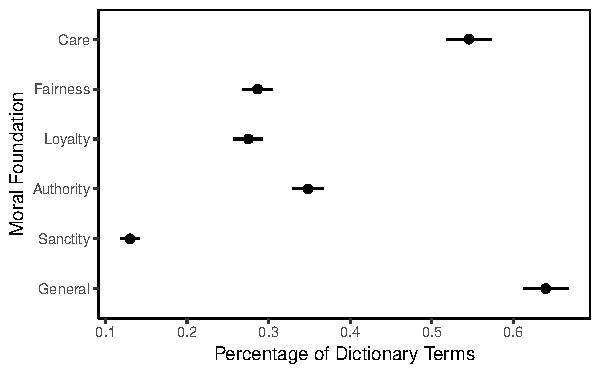
\includegraphics{/data/Dropbox/Uni/Projects/2017/cmv/calc/fig/mft_op_individual.pdf}
\caption[Moral Foundations in Paired Data]{Moral Foundations in Paired Data: Average percentage of dictionary terms relative to the total number of words in each original post starting a discussion (including 95\% confidence intervals).}
\end{figure}


\clearpage
\subsection{Distribution of MFT cosine similarity in Paired Data}

\begin{figure}[h]
\centering
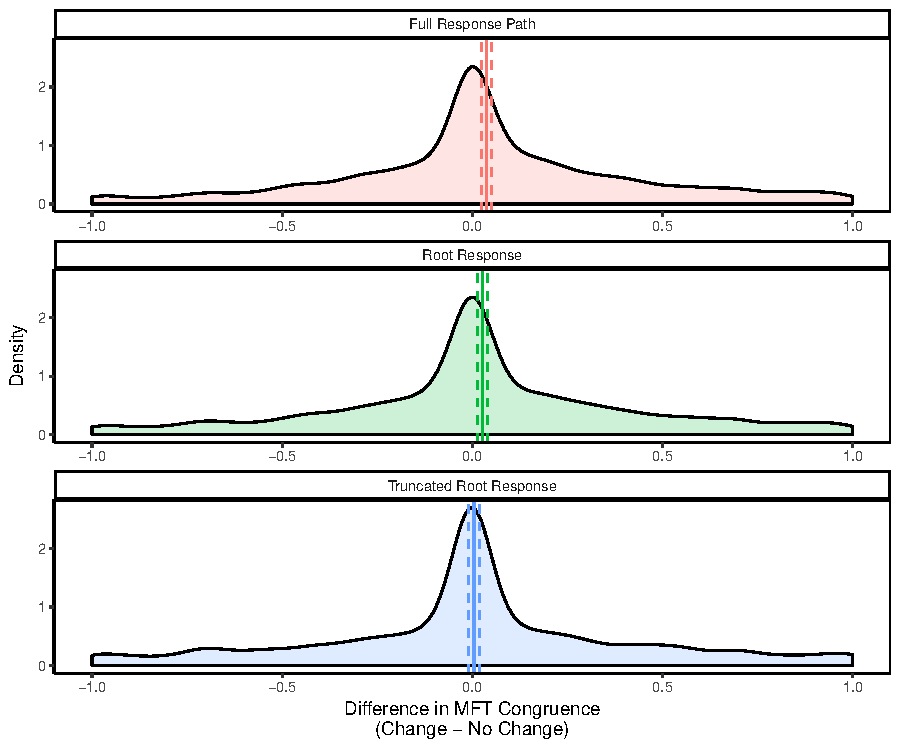
\includegraphics{/data/Dropbox/Uni/Projects/2017/cmv/calc/fig/cosine_density.pdf}
\caption{Distributions of the difference in MFT cosine similarity.}
\end{figure}


\begin{figure}[h]
\centering
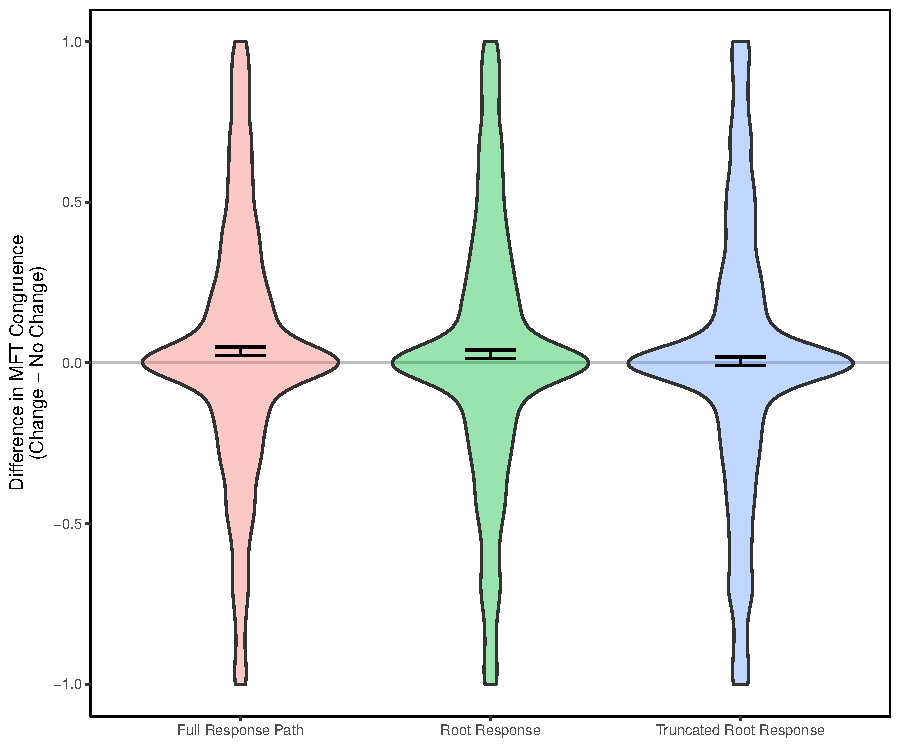
\includegraphics{/data/Dropbox/Uni/Projects/2017/cmv/calc/fig/cosine_violin.pdf}
\caption{Distributions of the difference in MFT cosine similarity (Violin Plot).}
\end{figure}

\clearpage
\section{Structural Topic Model Results}
\renewcommand\thefigure{B.\arabic{figure}}
\renewcommand\thetable{B.\arabic{table}}
\setcounter{figure}{0}
\setcounter{table}{0}

\subsection{Original Posts}

\begin{figure}[h]
\centering
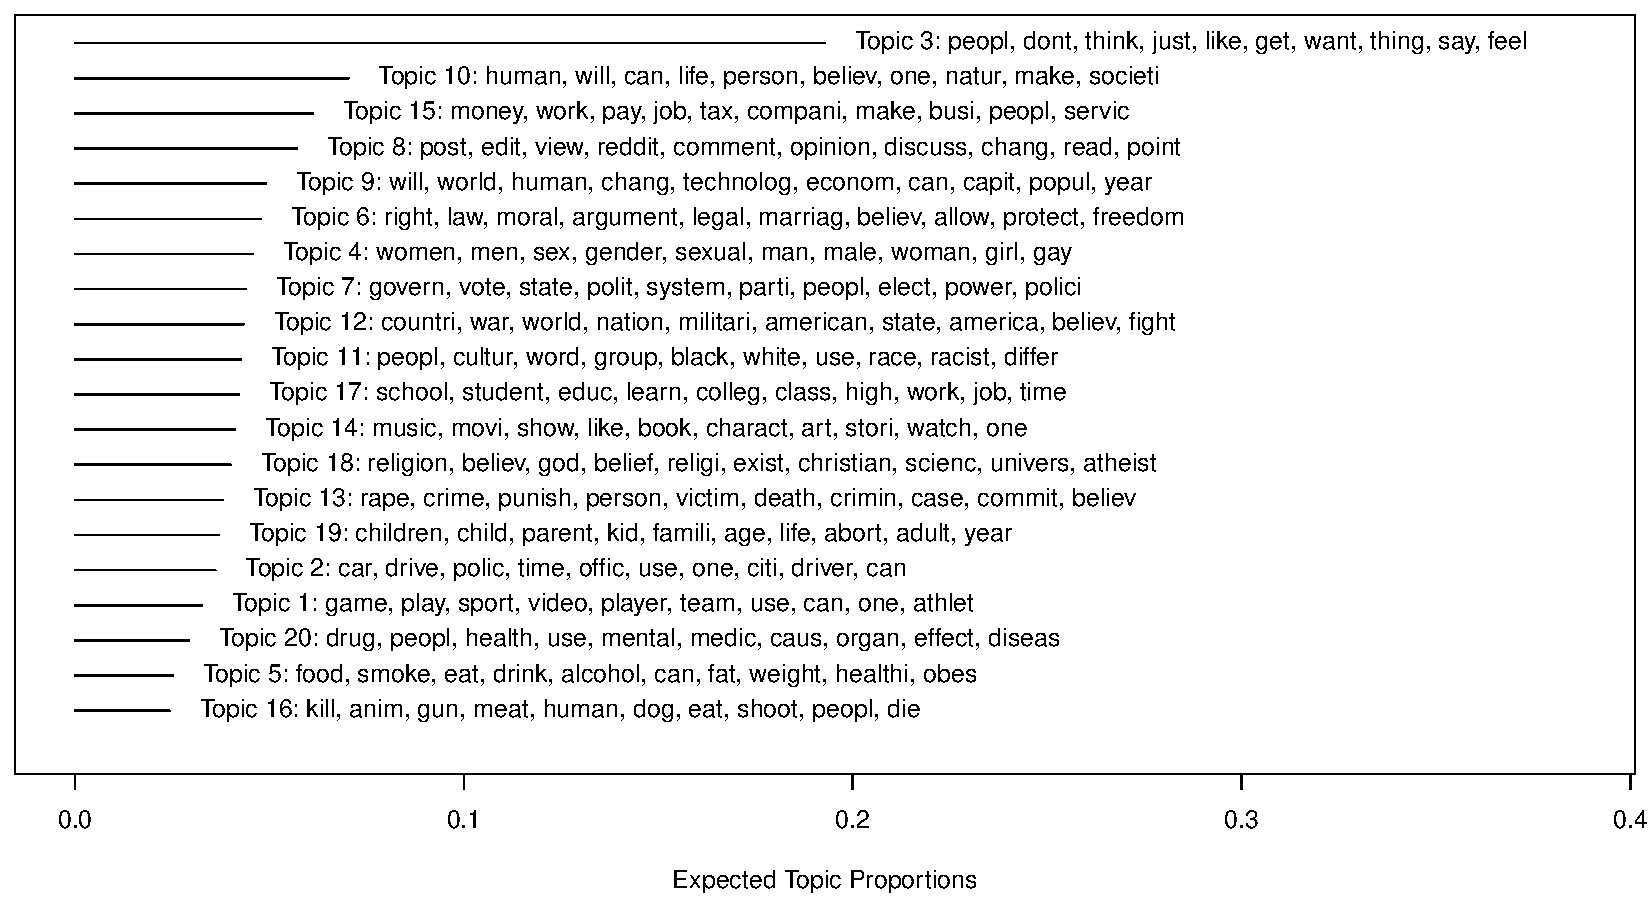
\includegraphics[width=\textwidth]{/data/Dropbox/Uni/Projects/2017/cmv/calc/fig/stm_op_prop.pdf}
\caption{Check description ch. 2}
\end{figure}

\begin{figure}[h]
\centering
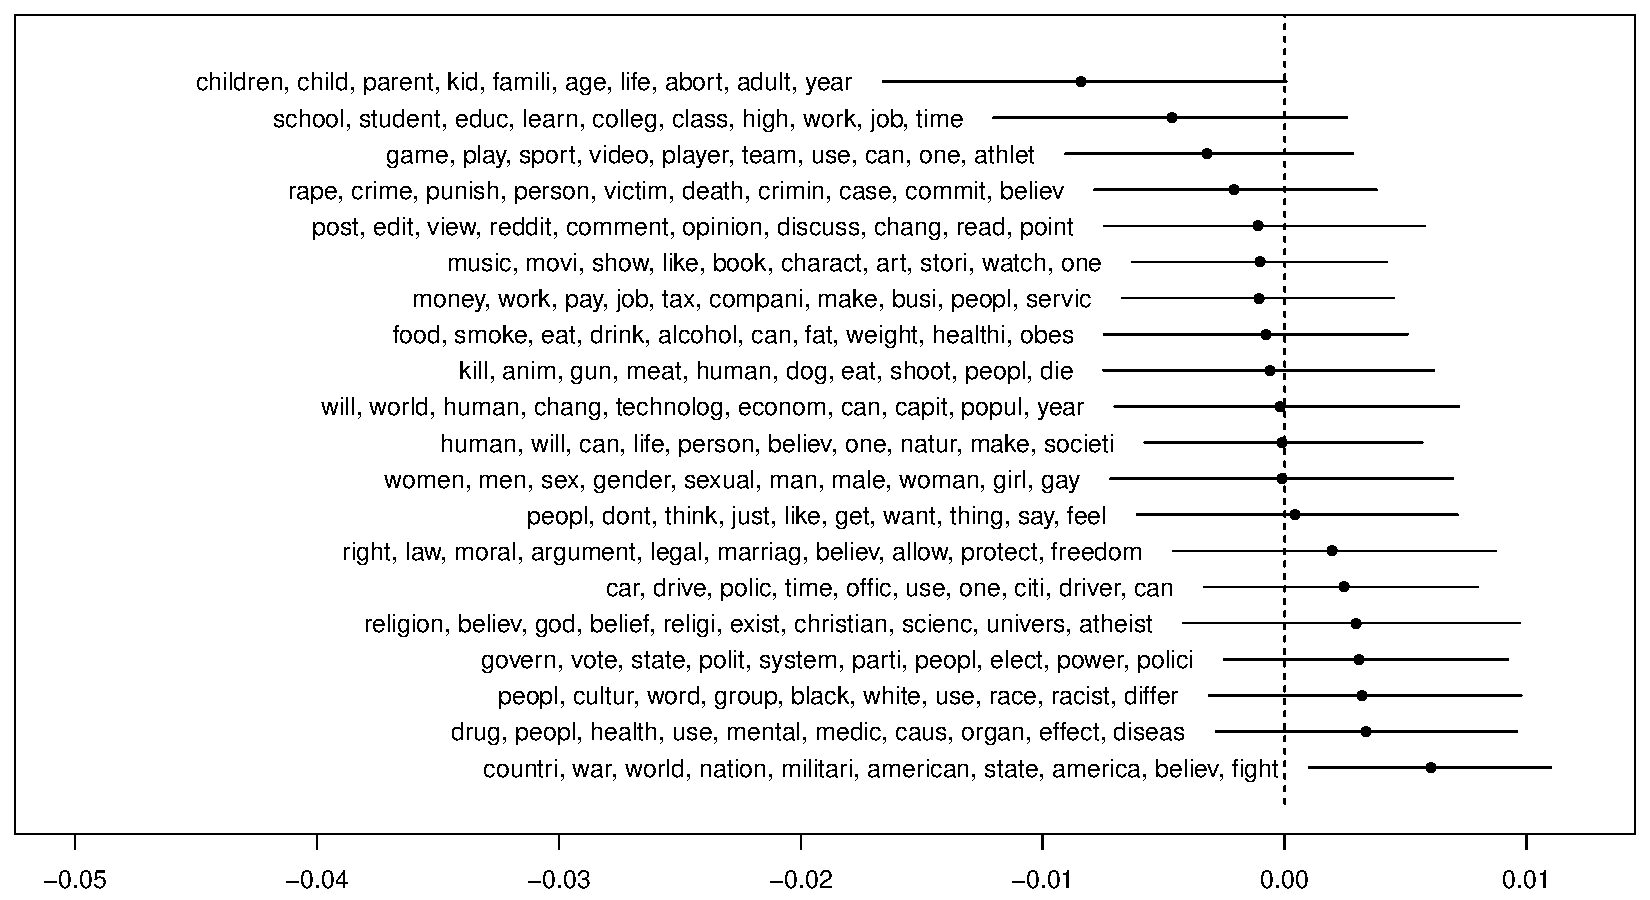
\includegraphics[width=\textwidth]{/data/Dropbox/Uni/Projects/2017/cmv/calc/fig/stm_op_diff.pdf}
\caption{Check description ch. 2}
\end{figure}

\clearpage
\subsection{Responses}

\begin{figure}[h]
\centering
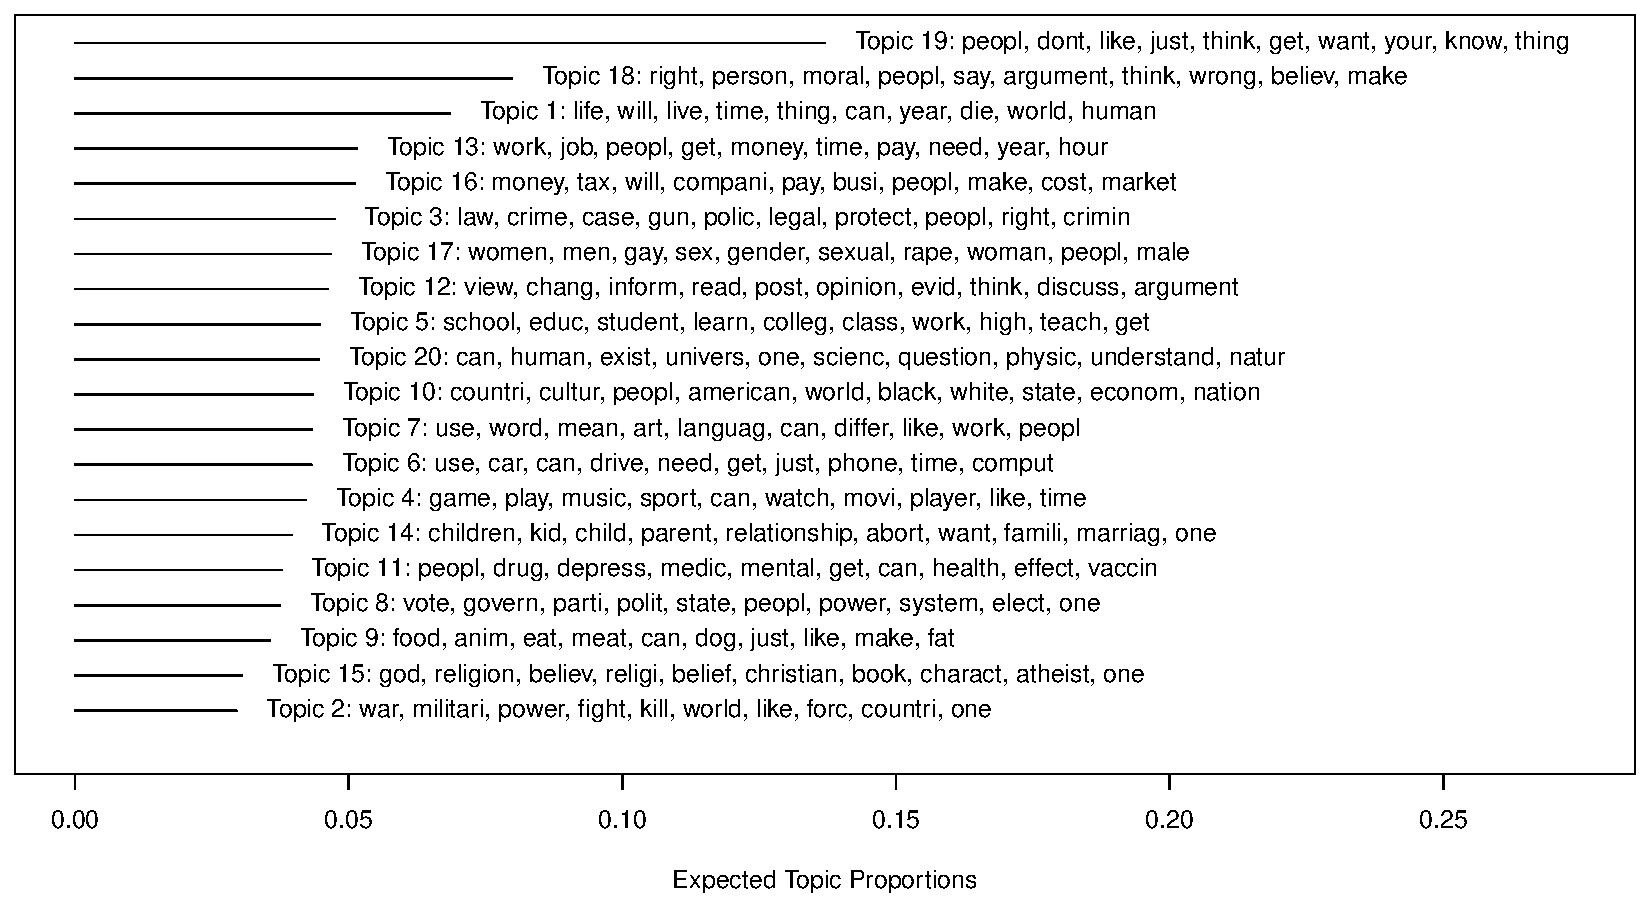
\includegraphics[width=\textwidth]{/data/Dropbox/Uni/Projects/2017/cmv/calc/fig/stm_pair_prop.pdf}
\caption{Check description ch. 2}
\end{figure}

\begin{figure}[h]
\centering
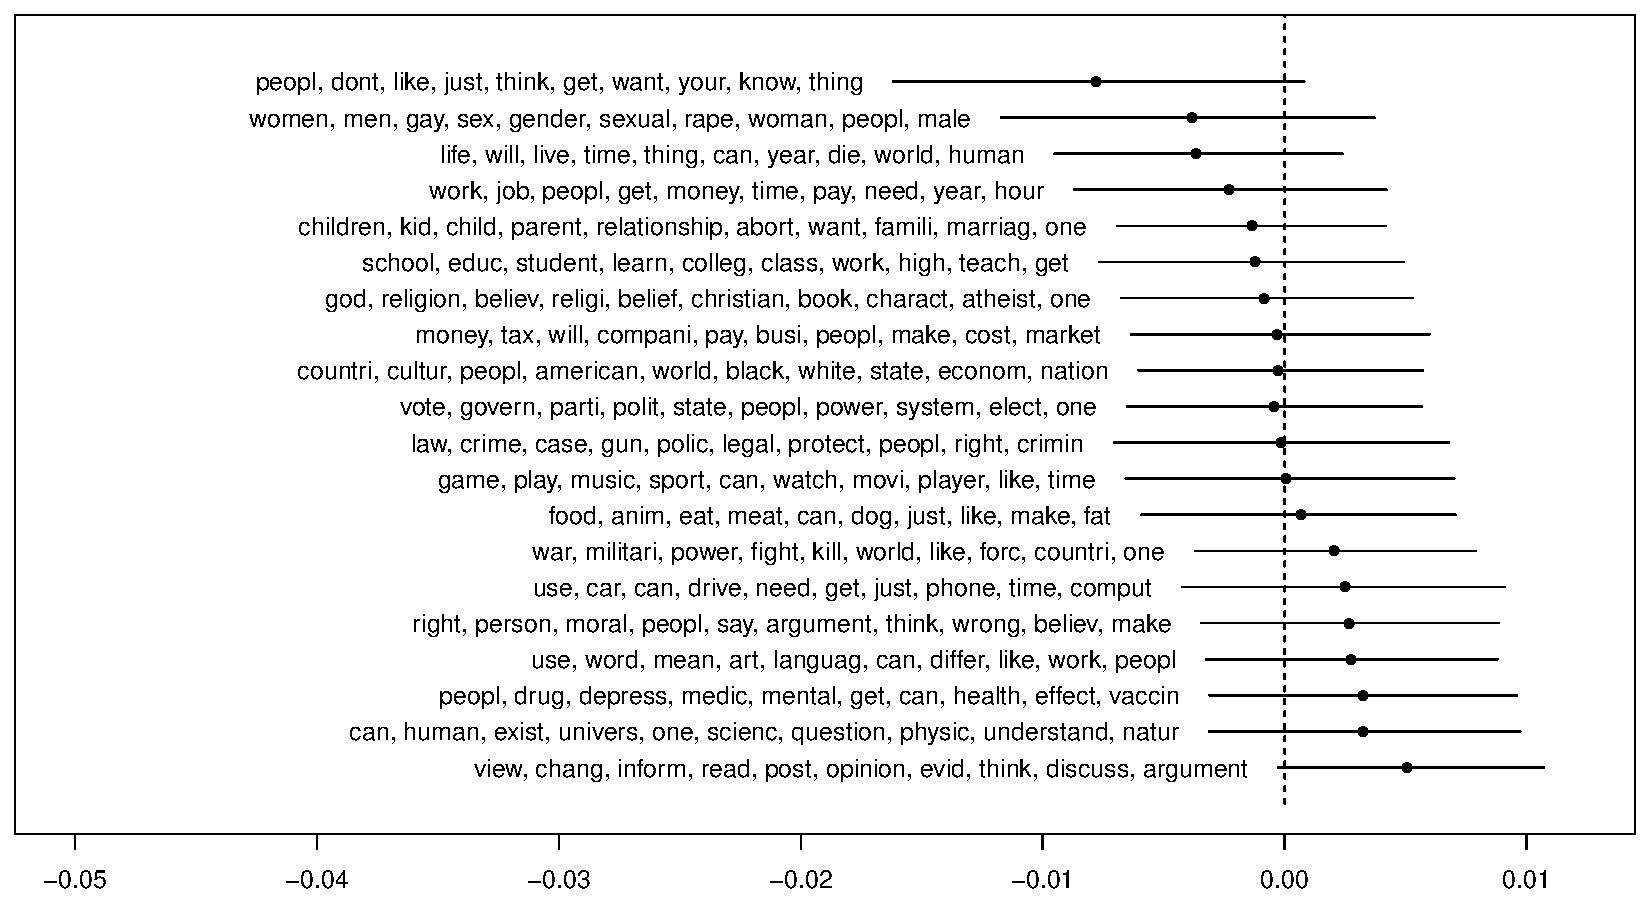
\includegraphics[width=\textwidth]{/data/Dropbox/Uni/Projects/2017/cmv/calc/fig/stm_pair_diff.pdf}
\caption{Check description ch. 2}
\end{figure}

